% !TeX spellcheck = en_US
% !TeX encoding = UTF-8
\chapter{Result}

\section{Assessment of Human Stress Levels}



\begin{figure}[h]
	\centering
	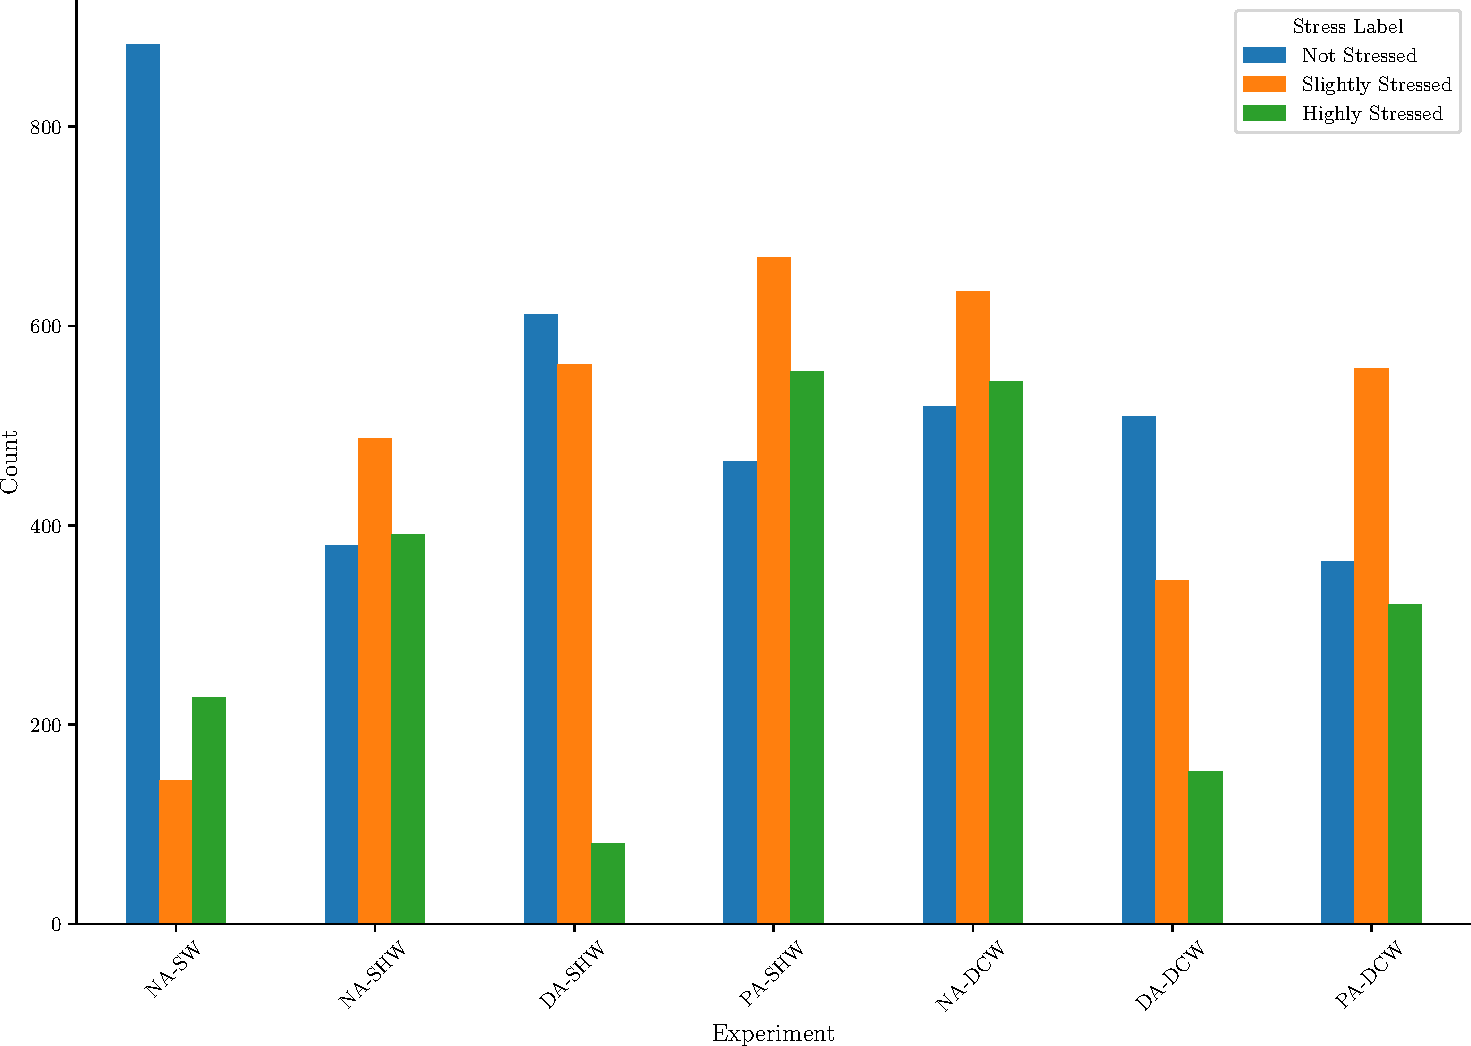
\includegraphics[width=0.9\columnwidth]{images/stress_levels_by_experiment2.pdf}
	\caption{Stress levels by experiment}
	\label{fig:result1}
\end{figure}

In this section, we present a comprehensive analysis of the perceived stress levels experienced by human participants in various our human-robot interaction scenarios. \autoref{fig:result1} shows the 3 different stress levels experienced by participants in each of the 7 different experimental setups.
Although in previous sections of our study we have used abbreviations such as AX, BX, and CX to refer to different experiment setups to match the protocol used for the data collection, for ease of understanding while presenting the results in this section we will adopt a more descriptive notation: 
\begin{itemize}
    \item\textbf{\gls{NA-SW}}
    \item\textbf{\gls{NA-SHW}}
    \item\textbf{\gls{DA-SHW}}
    \item\textbf{\gls{PA-SHW}}
    \item\textbf{\gls{NA-DCW}}
    \item\textbf{\gls{DA-DCW}}
    \item\textbf{\gls{PA-DCW}}
\end{itemize}


In the No Collision Avoidance in a Separated Workspace (NA-SW) scenario, the high prevalence of 'Not Stressed' responses is consistent with expectations that humans are most comfortable when working in an area separate from robots. Yet, the observation that 'High Stress' responses exceed those in scenarios with Dynamic Collision Avoidance in a Shared Workspace (DA-SHW) and Dynamic Collision Avoidance with Direct Collaboration in a Shared Workspace (DA-DCW) may initially appear contradictory. A potential rationale for this will be discussed subsequently.

For the No Collision Avoidance in a Shared Workspace (NA-SHW), there's a marked increase in stress levels, both 'Slightly Stressed' and 'Highly Stressed,' compared to the separated workspace (NA-SW). This is anticipated as sharing a workspace with robots, in the absence of any collision avoidance mechanisms, could lead to increased safety concerns and unpredictability, thereby elevating stress levels.

Another common pattern that can be seen is that introduction of Dynamic (DA) and Predictive (PA) Collision Avoidance strategies in both Shared Workspace (SHW) and Direct Collaboration (DCW) scenarios has generally led to a reduction in stress levels, with a particularly noticeable decrease in the DCW scenarios. However, this trend is not as apparent at first in the Predictive Collision Avoidance in a Shared Workspace (PA-SHW) scenario, where the number of 'Highly Stressed' instances is unexpectedly higher than in the scenario without collision avoidance (NA). It is important to consider that the overall count in the PA-SHW and No Collision Avoidance with Direct Collaboration in a Shared Workspace (NA-DCW) scenarios is higher than in other contexts, which may have influenced the stress results. The data shows the following count of instances for each task
NA-SW: 1254,
NA-SHW: 1258,
DA-SHW: 1255,
PA-SHW: 1687,
NA-DCW: 1698,
DA-DCW: 1007,
PA-DCW: 1242.
This discrepancy suggests that tasks PA-SHW and NA-DCW required more time for completion, potentially skewing the perceived stress levels.

Efforts were made to standardize each task's difficulty and completion time, but the tasks involving Predictive Collision Avoidance in a Shared Workspace (PA-SHW) and No Collision Avoidance with Direct Collaboration in a Shared Workspace (NA-DCW) inherently took longer, likely due to the task design that included attaching wheels to the base items at four separate locations.(Refer \autoref{fig:task}). 

Interestingly, another experiment that involved attaching wheels to base items was NA-SW. However, because there was no delay for the human to wait for the robot to deliver parts, this may have counteracted the longer task time. Nevertheless, the requirement of attaching wheels might have contributed to increased frustration levels, potentially explaining the slightly higher count of 'Highly Stressed' in the NA-SW scenario.

Interestingly, the tasks with the fewest attachment points—Dynamic Collision Avoidance in a Shared Workspace (DA-SHW) with five, and Dynamic Collision Avoidance with Direct Collaboration in a Shared Workspace (DA-DCW) with four—recorded the lowest counts of 'Highly Stressed' responses.

The diversity in task design was intentional to minimize the learning effects that could arise from performing similar tasks repeatedly. The goal was to create tasks that were distinct yet comparable in difficulty. The maximum number of attachment points was seven, with the minimum being four. However, it appears that this approach may have inadvertently introduced a variable of task complexity that was not adequately accounted for in the study's design.

Some other clear patterns shown are the increase of stress levels from the Dynamic collision avoidance (DA) to the Predictive collision avoidance (PA) in both the Shared workspace (SHW) and the Direct Collaboration (DCW) scenarios.

A potential explanation for this pattern is that the Predictive Collision Avoidance system may not be finely calibrated for the range of human actions during the item handover task. This lack of precise paramter tuning leads to unpredictability in the robot's actions, which are based on future projections. The added complexity of the robot's behavior can contribute to higher stress levels for the human workers.

During the experiments, variations in human behavior were observed. Some participants simply extended their hands to the robot for the handover, while others leaned in with their entire body, prompting the robot to misinterpret the action as a potential collision and retreat from the handover point for safety reasons. This forces the human to revert to their original position and attempt the handover again, leading to potential frustration and increased stress.

It's important to note that the optimization of the Predictive Collision Avoidance system's parameters was conducted prior to data collection, considering only a single standard behavior rather than the diverse behaviors of different participants. Future work could focus on refining the system to accommodate a wider range of human behaviors during handover tasks. Additionally, a hybrid approach that utilizes Predictive Collision Avoidance for general tasks and switches to Dynamic Collision Avoidance for handovers is proposed as a potential solution to reduce stress. This approach is further discussed in the \autoref{sec:futurework}.


\section{Machine Learning Classification Models} 
In the evaluation of stress detection models, several machine learning algorithms were compared.
\subsection*{Support Vector Machine}
Specifically, Support Vector Machine (SVM) models with various kernel functions were employed. For the SVM with Linear Kernel, a linear kernel was utilized with a regularization parameter (C) set to 1.0, enabling probability estimation. The SVM with Polynomial Kernel employed a polynomial kernel of degree 3, also with a regularization parameter of 1.0 and probability estimation enabled. Additionally, the SVM with Radial Basis Function (RBF) Kernel utilized an RBF kernel with a regularization parameter of 1.0 and a gamma value of 0.1 for the kernel coefficient, allowing for probability estimation. Lastly, the SVM with Sigmoid Kernel employed a sigmoid kernel with a regularization parameter of 1.0 and a coefficient of 0.0. All models underwent evaluation using a 10-fold cross-validation technique. Detailed results, including mean scores and confusion matrices, can be found in \autoref{tab:scores} and Figures 1-4, respectively.

\begin{table}[hhtbp]
    \centering
    \begin{tabular}{|l|c|c|c|c|c|}
    \hline
    \textbf{Model} & \textbf{Accuracy} & \textbf{F1 Score} & \textbf{Precision} & \textbf{Recall} & \textbf{AUC} \\ \hline
    \textbf{SVM with Linear Kernel} & 0.628 & 0.622 & 0.630 & 0.628 & 0.805 \\
    \textbf{SVM with Polynomial Kernel } & 0.750 & 0.745 & 0.803 & 0.750 & 0.946 \\
    \textbf{SVM with RBF Kernel} & \textbf{0.916} & \textbf{0.915} & \textbf{0.926} & \textbf{0.916} & \textbf{0.994} \\
    \textbf{SVM with Sigmoid Kernel} & 0.445 & 0.440 & 0.449 & 0.445 & 0.599 \\ \hline
    \end{tabular}
    \caption{Mean Scores for SVM Models with K-Fold Cross-Validation ($k=10$)}
    \label{tab:scores}
    \end{table}
    

    \begin{figure}[htbp]
        \centering
        \begin{minipage}[b]{0.40\textwidth}
          \centering
          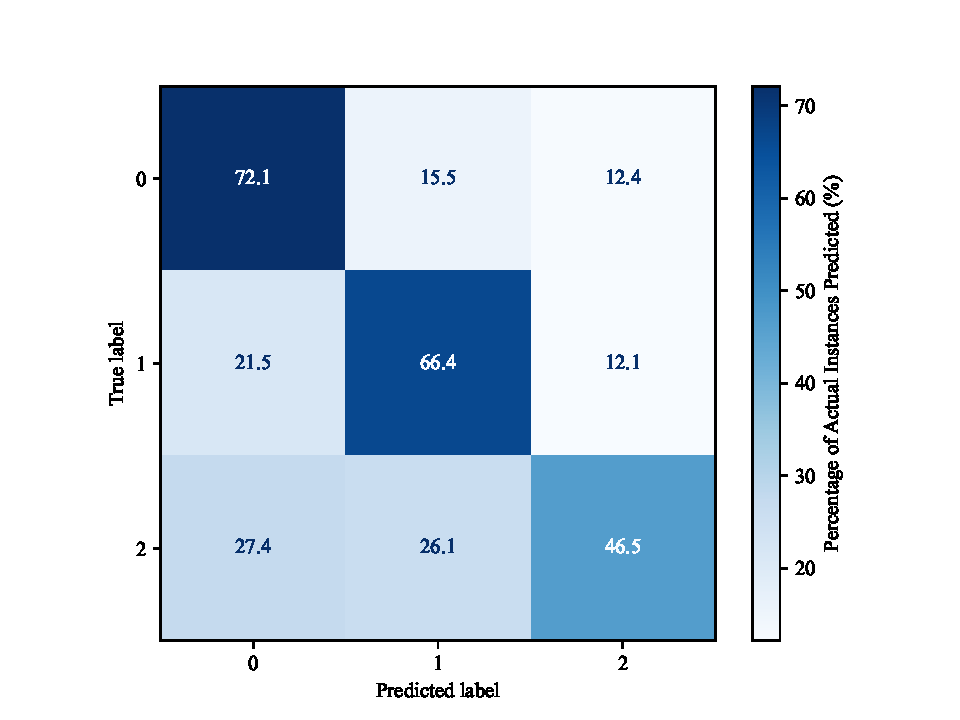
\includegraphics[width=\textwidth]{images/confusion_matrix_linear_svm.pdf}
          \caption{Confusion Matrix for Linear SVM}
          \label{fig:confusion_linear}
        \end{minipage}
        \hfill
        \begin{minipage}[b]{0.45\textwidth}
          \centering
          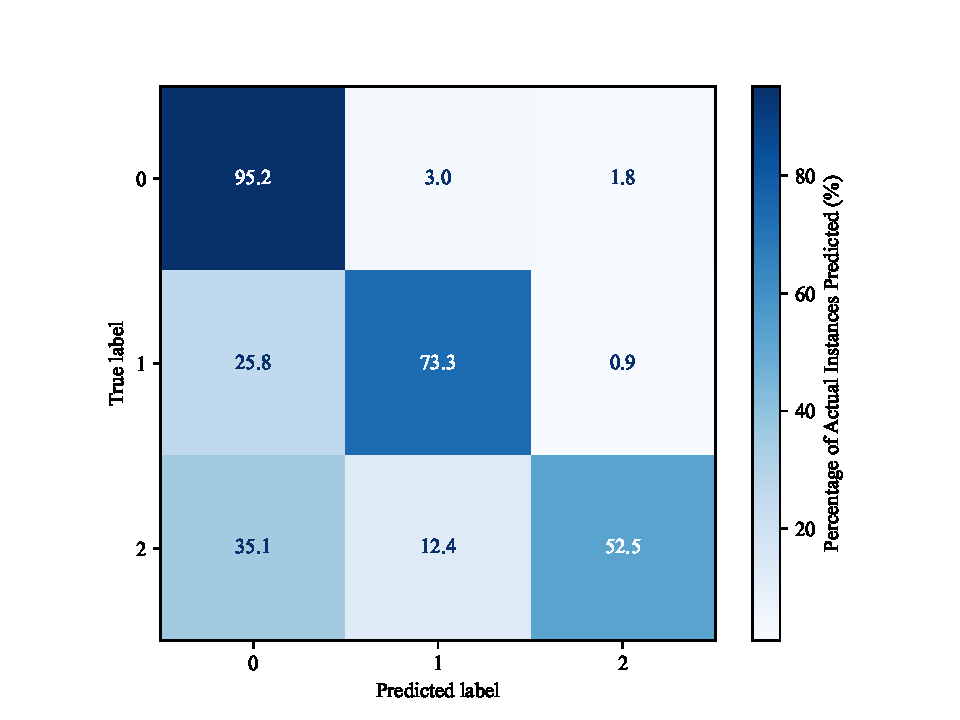
\includegraphics[width=\textwidth]{images/confusion_matrix_poly_svm.pdf}
          \caption{Confusion Matrix for Polynomial SVM}
          \label{fig:confusion_poly}
        \end{minipage}
        \end{figure}
        
        \begin{figure}[htbp]
        \centering
        \begin{minipage}[b]{0.45\textwidth}
          \centering
          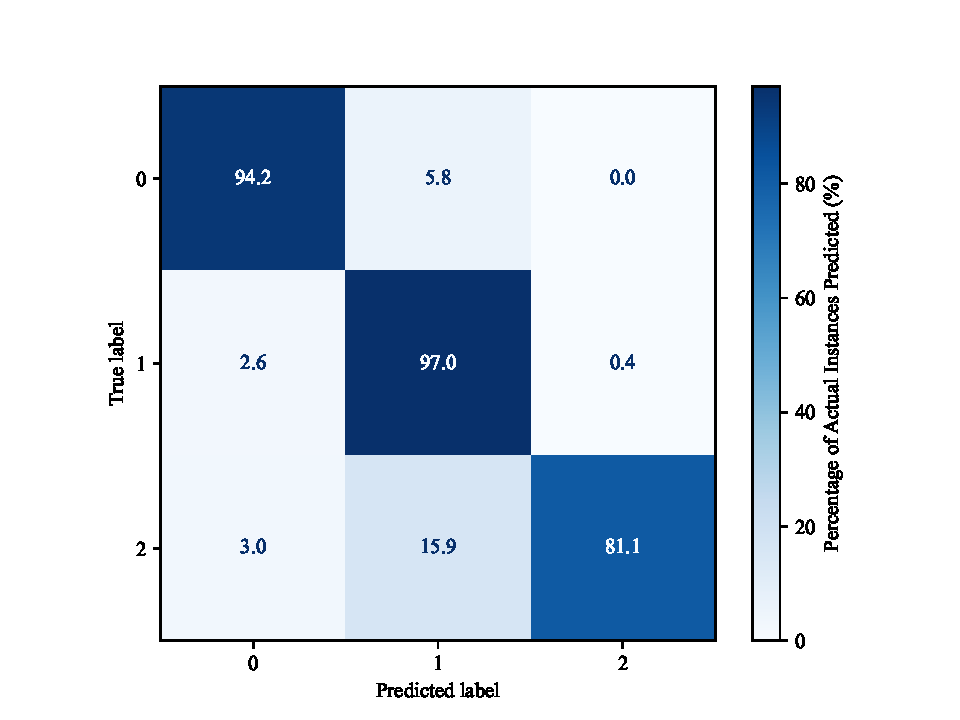
\includegraphics[width=\textwidth]{images/confusion_matrix_rbf.pdf}
          \caption{Confusion Matrix for RBF SVM}
          \label{fig:confusion_rbf}
        \end{minipage}
        \hfill
        \begin{minipage}[b]{0.45\textwidth}
          \centering
          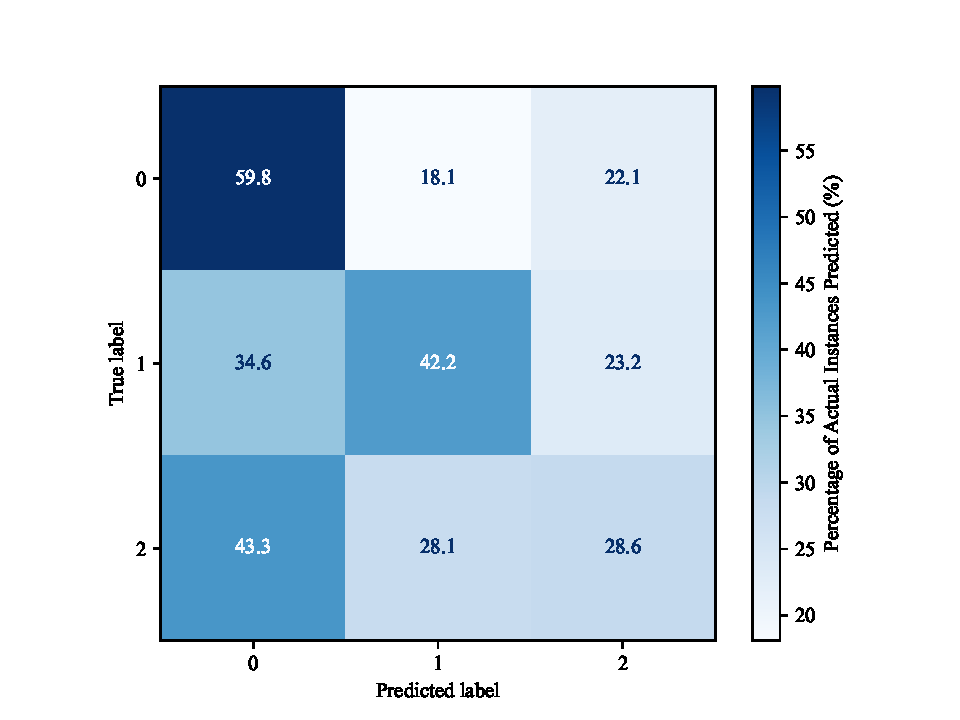
\includegraphics[width=\textwidth]{images/confusion_matrix_sigmoid_svm.pdf}
          \caption{Confusion Matrix for Sigmoid SVM}
          \label{fig:confusion_sigmoid}
        \end{minipage}
        \end{figure}
        
Among the models, the SVM with RBF Kernel achieved the highest mean scores across all metrics, including AUC, accuracy, F1 score, precision, and recall. This performance may be attributed to the RBF kernel's ability to capture non-linear relationships in the data effectively. 



\subsection*{Random Forest}
The results obtained from Random Forest models with different numbers of trees (n\_estimators) are shown in \autoref{tab:rf_scores}

\begin{table}[htbp]
    \centering
    \begin{tabular}{|p{5cm}|c|c|c|c|c|}
    \hline
    \textbf{Model} & \textbf{Accuracy} & \textbf{F1 Score} & \textbf{Precision} & \textbf{Recall} & \textbf{AUC} \\ \hline
    \textbf{Random Forest (n\_estimators=100)} & 0.949 & 0.949 & 0.950 & 0.949 & 0.992 \\
    \textbf{Random Forest (n\_estimators=200)} & 0.949 & 0.949 & 0.950 & 0.949 & 0.993 \\ \hline
    \end{tabular}
    \caption{Mean Scores for Random Forest Models with Different Numbers of Estimators}
    \label{tab:rf_scores}
\end{table}

    
    This table presen



\subsection*{Naive Bayes}
The Gaussian Naive Bayes classifier, with its assumption of feature independence, yielded moderate performance across various metrics, as shown in Table \ref{tab:nb_scores}. 

\begin{table}[hhtbp]
    \centering
    \begin{tabular}{|l|c|c|c|c|c|}
    \hline
    \textbf{Model} & \textbf{Accuracy} & \textbf{F1 Score} & \textbf{Precision} & \textbf{Recall} & \textbf{AUC} \\
    \hline
    \textbf{Gaussian Naive Bayes} & 0.532 & 0.507 & 0.550 & 0.532 & 0.702 \\
    \hline
    \end{tabular}
    \caption{Mean Scores for Gaussian Naive Bayes with K-Fold Cross-Validation ($k=10$)}
    \label{tab:nb_scores}
    \end{table}



\subsection*{k-Nearest Neighbors (k-NN)}
In this study, the k-Nearest Neighbors (k-NN) algorithm was utilized with varying values of the parameter k. The default distance metric used by k-NN, Euclidean distance, was employed for calculating the proximity between data points. Four different configurations of the k-NN model were examined, with k values set to 5, 10, 15, and 20, respectively. Each k-NN model underwent a 10-fold cross-validation procedure for evaluation. The results, including mean scores and confusion matrices, are presented in \autoref{tab:knn_scores} and Figures 5-8, respectively.

\begin{table}[hhtbp]
    \centering
    \begin{tabular}{|l|c|c|c|c|c|}
    \hline
    \textbf{Model} & \textbf{Accuracy} & \textbf{F1 Score} & \textbf{Precision} & \textbf{Recall} & \textbf{AUC} \\ \hline
    \textbf{k-NN (k=5)} & \textbf{0.909} & \textbf{0.909} & \textbf{0.913} & \textbf{0.909} & \textbf{0.982} \\
    \textbf{k-NN (k=10)} & 0.833 & 0.833 & 0.844 & 0.833 & 0.954 \\
    \textbf{k-NN (k=15)} & 0.780 & 0.779 & 0.795 & 0.780 & 0.924 \\
    \textbf{k-NN (k=20)} & 0.780 & 0.779 & 0.795 & 0.780 & 0.924 \\ \hline
    \end{tabular}
    \caption{Mean Scores for k-NN Models with K-Fold Cross-Validation ($k=10$)}
    \label{tab:knn_scores}
\end{table}

\begin{figure}[htbp]
    \centering
    \begin{minipage}[b]{0.45\textwidth}
        \centering
        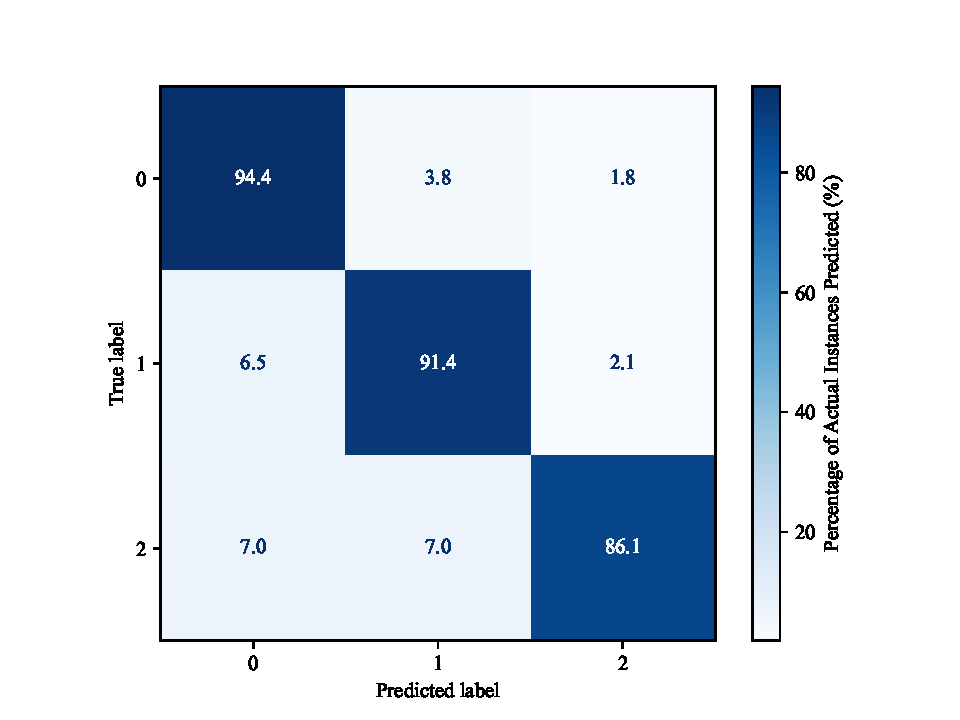
\includegraphics[width=\textwidth]{images/confusion_matrix_knn5.pdf}
        \caption{Confusion Matrix for k-NN (k=5)}
        \label{fig:confusion_knn_5}
    \end{minipage}
    \hfill
    \begin{minipage}[b]{0.45\textwidth}
        \centering
        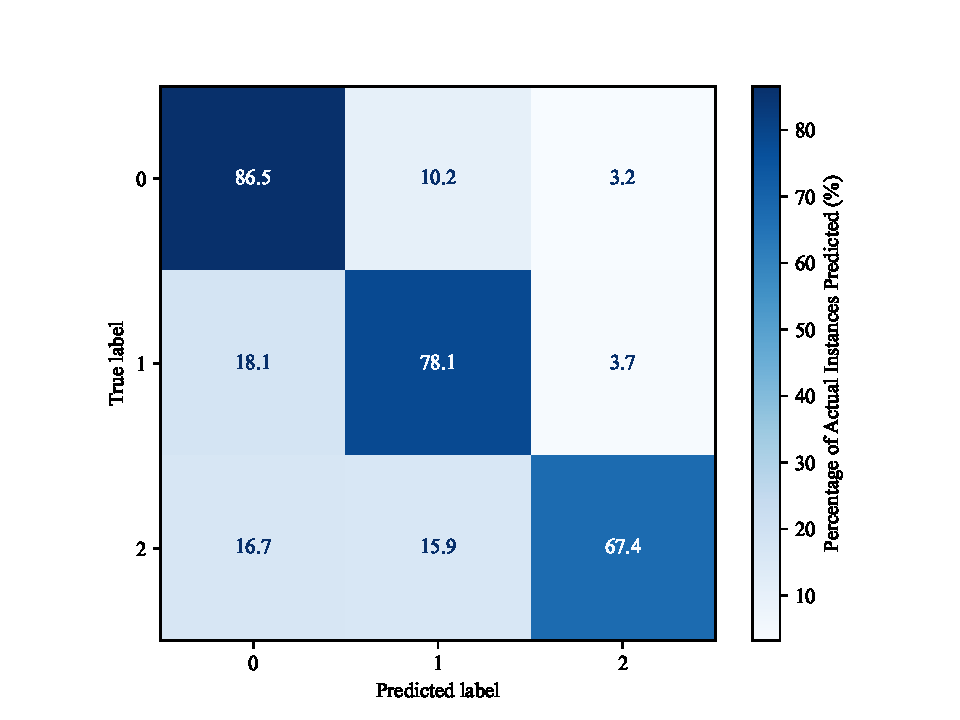
\includegraphics[width=\textwidth]{images/confusion_matrix_knn10.pdf}
        \caption{Confusion Matrix for k-NN (k=10)}
        \label{fig:confusion_knn_10}
    \end{minipage}
\end{figure}

\begin{figure}[htbp]
    \centering
    \begin{minipage}[b]{0.45\textwidth}
        \centering
        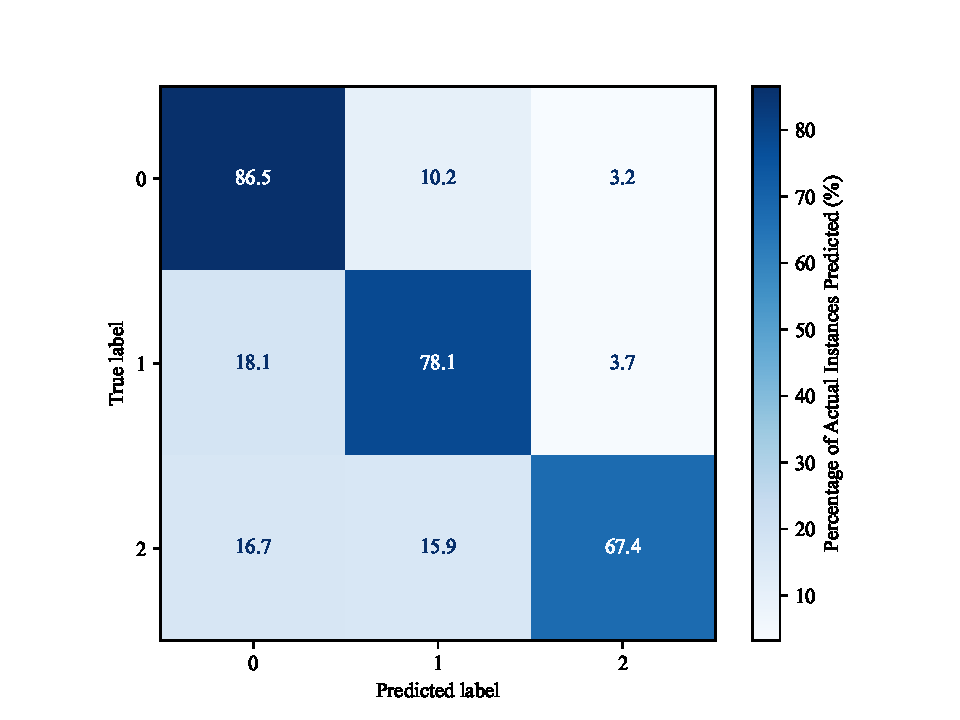
\includegraphics[width=\textwidth]{images/confusion_matrix_knn15.pdf}
        \caption{Confusion Matrix for k-NN (k=15)}
        \label{fig:confusion_knn_15}
    \end{minipage}
    \hfill
    \begin{minipage}[b]{0.45\textwidth}
        \centering
        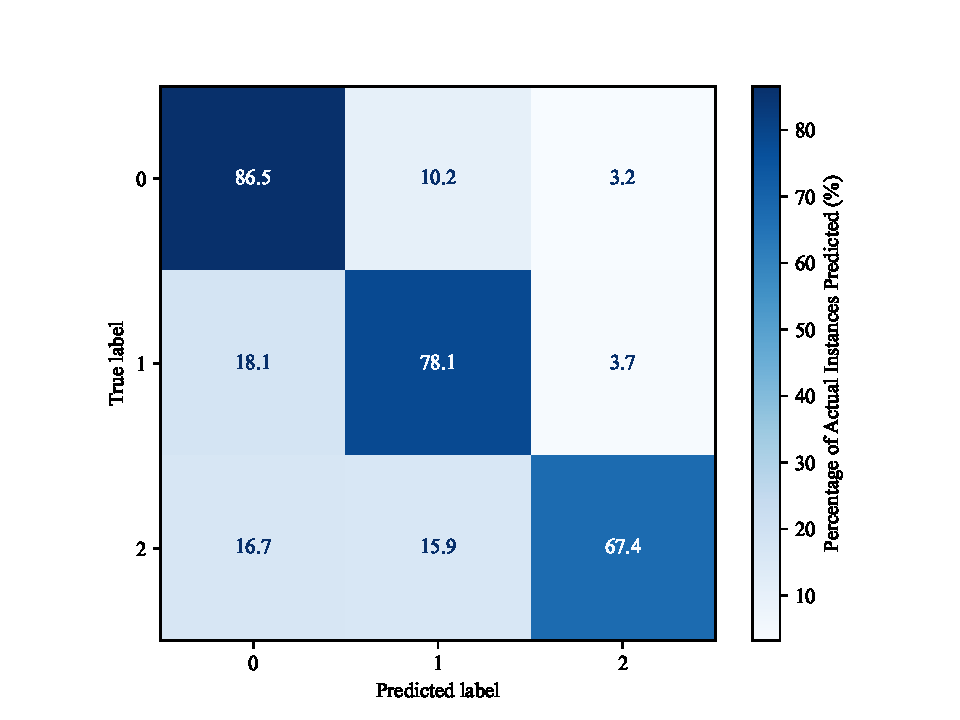
\includegraphics[width=\textwidth]{images/confusion_matrix_knn20.pdf}
        \caption{Confusion Matrix for k-NN (k=20)}
        \label{fig:confusion_knn_20}
    \end{minipage}
\end{figure}

\subsection*{AdaBoost}
The AdaBoost models were trained using the AdaBoost classifier with varying numbers of estimators. Specifically, the models were configured with 50, 100, 150, and 200 estimators. The results, summarized in Table \ref{tab:adaboost_scores}.


\begin{table}[hhtbp]
    \centering
    \begin{tabular}{|l|c|c|c|c|c|}
    \hline
    \textbf{Model} & \textbf{Accuracy} & \textbf{F1 Score} & \textbf{Precision} & \textbf{Recall} & \textbf{AUC} \\ \hline
    \textbf{Adaboost (Estimators=50)} & 0.647 & 0.644 & 0.653 & 0.647 & 0.814 \\
    \textbf{Adaboost (Estimators=100)} & 0.702 & 0.701 & 0.708 & 0.702 & 0.829 \\
    \textbf{Adaboost (Estimators=150)} & 0.720 & 0.718 & 0.724 & 0.720 & 0.844 \\
    \textbf{Adaboost (Estimators=200)} & 0.732 & 0.731 & 0.736 & 0.732 & 0.849 \\ \hline
    \end{tabular}
    \caption{Mean Scores for AdaBoost Models with Different Numbers of Estimators}
    \label{tab:adaboost_scores}
    \end{table}
    
    \begin{figure}[htbp]
        \centering
        \begin{minipage}[b]{0.45\textwidth}
        \centering
        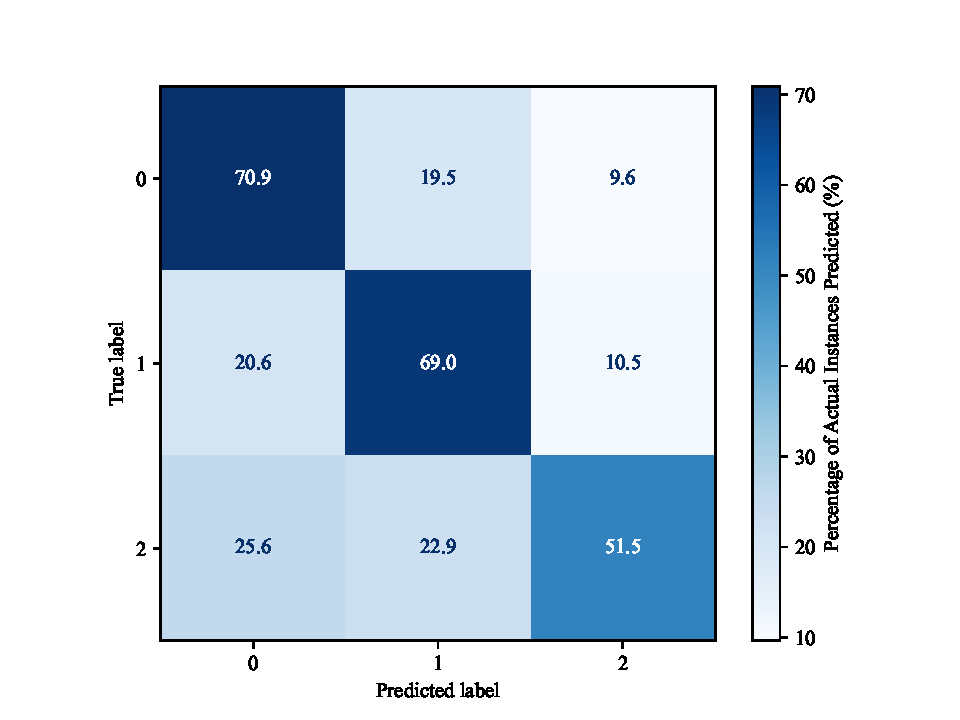
\includegraphics[width=\textwidth]{images/confusion_matrix_adaboost50.pdf}
        \caption{Confusion Matrix for AdaBoost (Estimators=50)}
        \label{fig:confusion_adaboost_50}
        \end{minipage}
        \hfill
        \begin{minipage}[b]{0.45\textwidth}
        \centering
        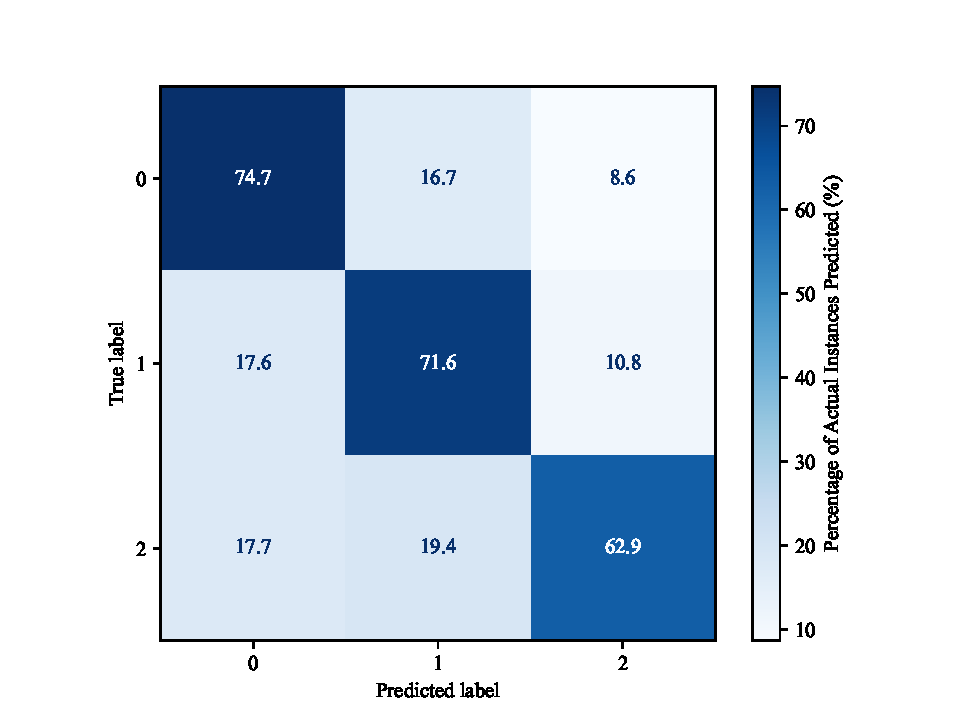
\includegraphics[width=\textwidth]{images/confusion_matrix_adaboost100.pdf}
        \caption{Confusion Matrix for AdaBoost (Estimators=100)}
        \label{fig:confusion_adaboost_100}
        \end{minipage}
        \end{figure}
        
        \begin{figure}[htbp]
        \centering
        \begin{minipage}[b]{0.45\textwidth}
        \centering
        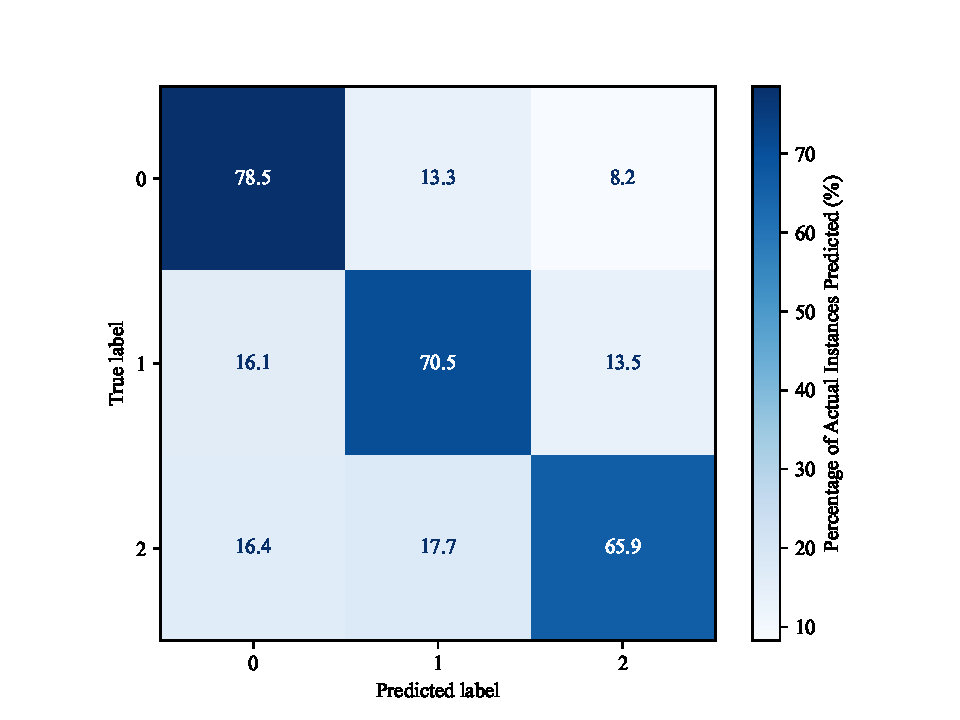
\includegraphics[width=\textwidth]{images/confusion_matrix_adaboost150.pdf}
        \caption{Confusion Matrix for AdaBoost (Estimators=150)}
        \label{fig:confusion_adaboost_150}
        \end{minipage}
        \hfill
        \begin{minipage}[b]{0.45\textwidth}
        \centering
        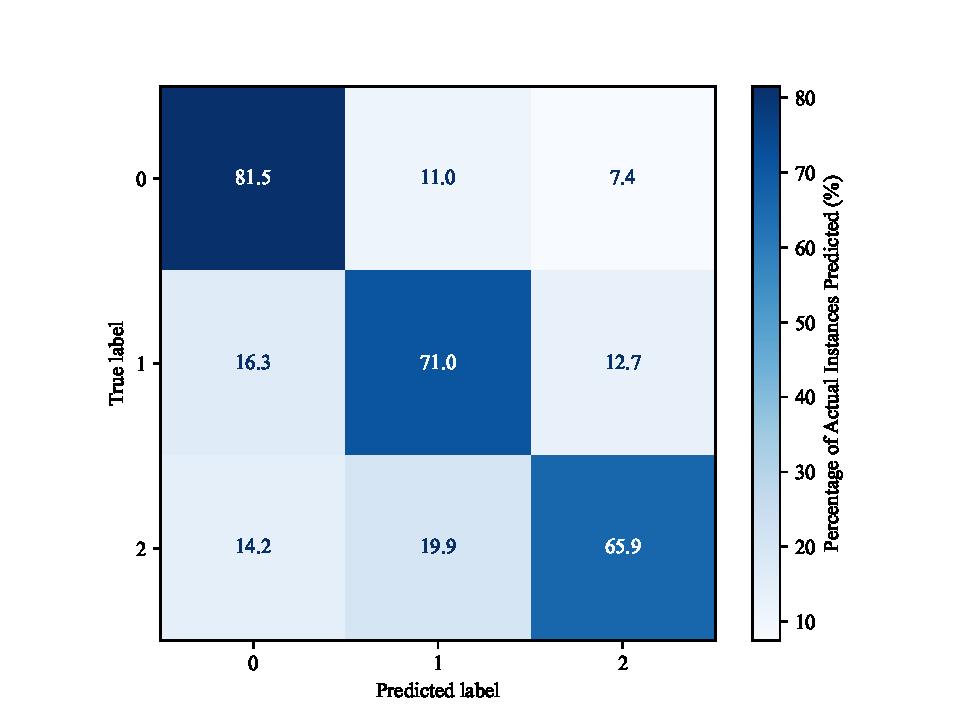
\includegraphics[width=\textwidth]{images/confusion_matrix_adaboost200.pdf}
        \caption{Confusion Matrix for AdaBoost (Estimators=200)}
        \label{fig:confusion_adaboost_200}
        \end{minipage}
        \end{figure}



\subsection*{Neural Netwrok -MLP}
Four MLP classifiers were trained with varying parameters to explore their impact on performance. The parameters used for each classifier are detailed in Table \ref{tab:mlp_params}. MLP-1 utilized a hidden layer size of 200 neurons, while MLP-2 had a hidden layer size of 100 neurons. Both MLP-1 and MLP-2 employed the Rectified Linear Unit (ReLU) activation function and the Adam solver, with an alpha value of 0.0008 and a maximum of 400 iterations. Additionally, MLP-3 and MLP-4 utilized logistic activation functions.

The mean scores for the MLP classifiers are presented in Table \ref{tab:mlp_scores}. Notably, MLP-3 achieved the highest accuracy, F1 score, precision, recall, and Area Under the Curve (AUC) among all models, indicating superior performance.

\begin{table}[hhtbp]
    \centering
    \begin{tabular}{|c|c|c|c|c|c|}
    \hline
    \textbf{Model} & \textbf{Hidden Layer Sizes} & \textbf{Activation} & \textbf{Solver} & \textbf{Alpha} & \textbf{Max Iter}  \\
    \hline
    MLP-1 & (200,) & ReLU & adam & 0.0008 & 400  \\
    MLP-2 & (100,) & ReLU & adam & 0.0008 & 400  \\
    MLP-3 & (100,) & Logistic & adam & 0.0008 & 400  \\
    MLP-4 & (200,) & Logistic & adam & 0.0008 & 400  \\
    \hline
    \end{tabular}
    \caption{Parameters Used for MLP Classifiers}
    \label{tab:mlp_params}
    \end{table}
    
    \begin{table}[hhtbp]
    \centering
    \begin{tabular}{|l|c|c|c|c|c|}
    \hline
    \textbf{Model} & \textbf{Accuracy} & \textbf{F1 Score} & \textbf{Precision} & \textbf{Recall} & \textbf{AUC} \\
    \hline
    MLP-1 & 0.894 & 0.894 & 0.895 & 0.894 & 0.972 \\
    MLP-2 & 0.889 & 0.889 & 0.891 & 0.889 & 0.969 \\
    MLP-3 & \textbf{0.922} & \textbf{0.922} & \textbf{0.924} & \textbf{0.922} & \textbf{0.987} \\
    MLP-4 & 0.909 & 0.909 & 0.910 & 0.909 & 0.982 \\
    
    \hline
    \end{tabular}
    \caption{Mean Scores for MLP Classifiers}
    \label{tab:mlp_scores}
    \end{table}
    
    \begin{figure}[htbp]
        \centering
        \begin{minipage}[b]{0.45\textwidth}
            \centering
            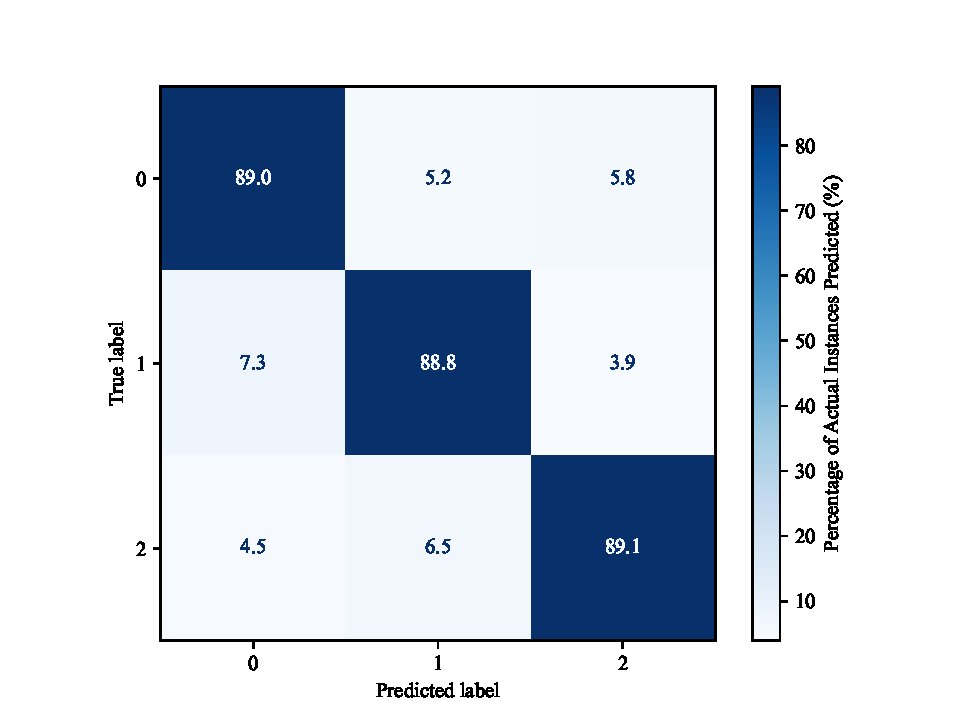
\includegraphics[width=\textwidth]{images/confusion_matrix_mlp200.pdf}
            \caption{Confusion Matrix for MLP-1}
            \label{fig:confusion_mlp_1}
        \end{minipage}
        \hfill
        \begin{minipage}[b]{0.45\textwidth}
            \centering
            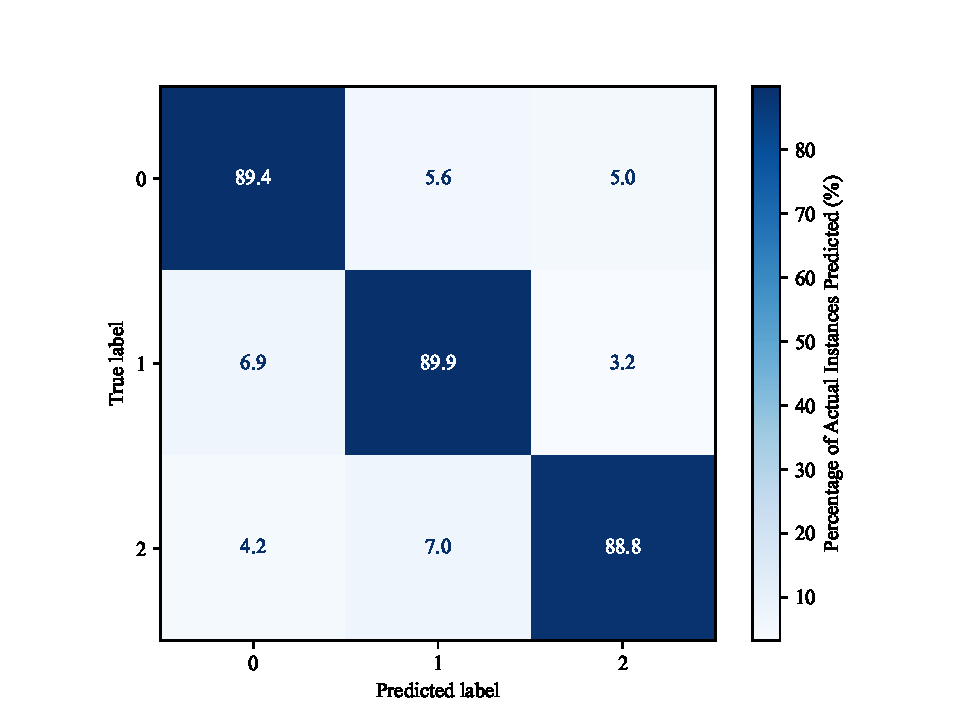
\includegraphics[width=\textwidth]{images/confusion_matrix_mlp100.pdf}
            \caption{Confusion Matrix for MLP-2}
            \label{fig:confusion_mlp_2}
        \end{minipage}
    \end{figure}
    
    \begin{figure}[htbp]
        \centering
        \begin{minipage}[b]{0.45\textwidth}
            \centering
            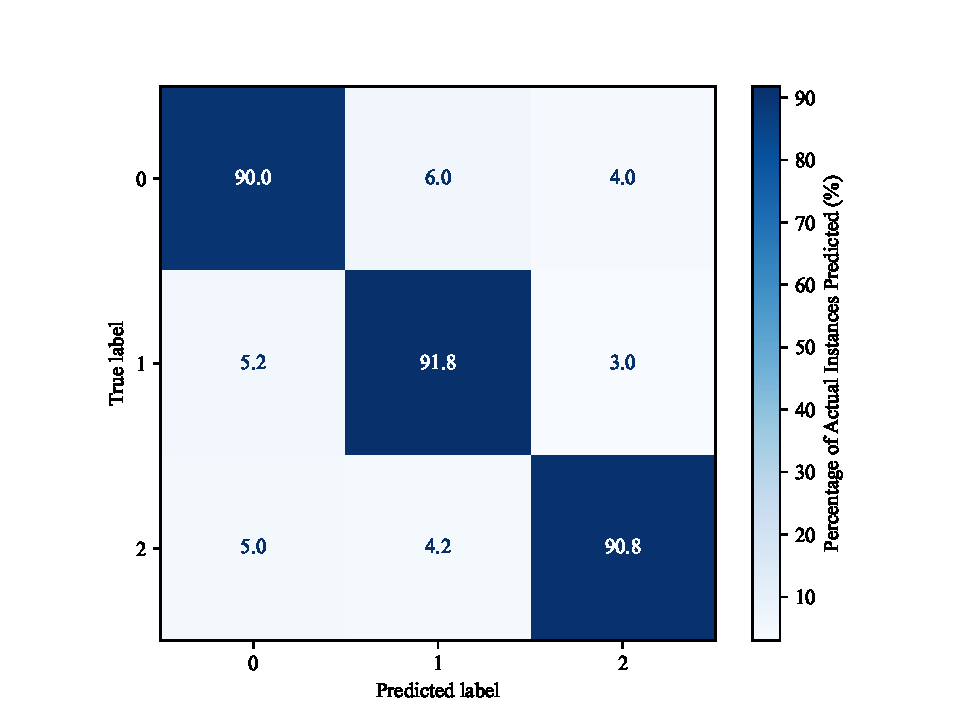
\includegraphics[width=\textwidth]{images/confusion_matrix_mlp100log.pdf}
            \caption{Confusion Matrix for MLP-3}
            \label{fig:confusion_mlp_3}
        \end{minipage}
        \hfill
        \begin{minipage}[b]{0.45\textwidth}
            \centering
            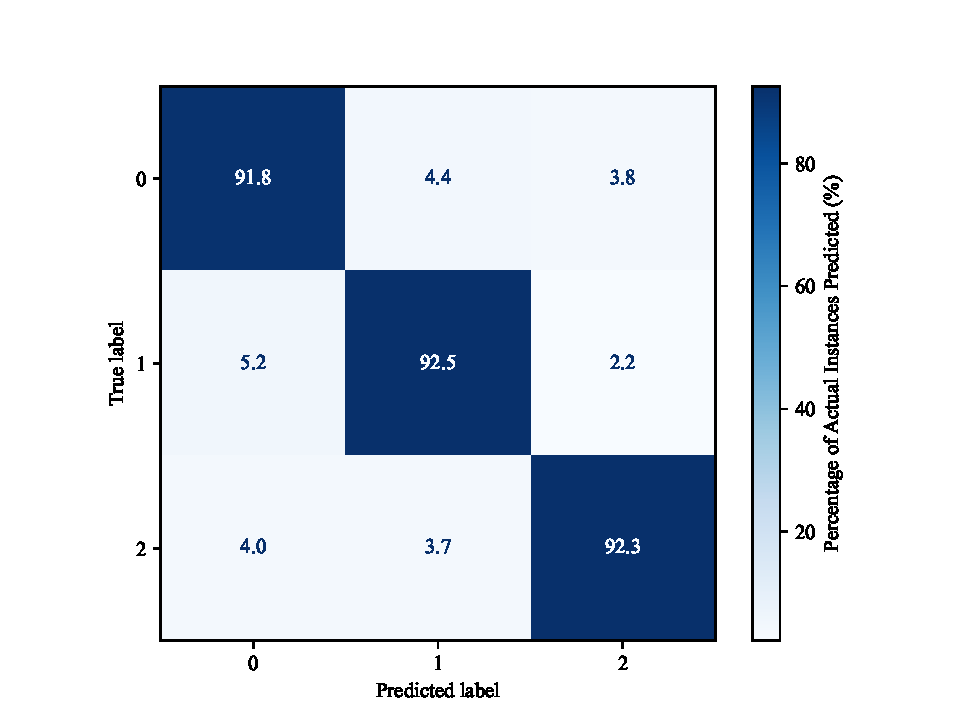
\includegraphics[width=\textwidth]{images/confusion_matrix_mlp200log.pdf}
            \caption{Confusion Matrix for MLP-4}
            \label{fig:confusion_mlp_4}
        \end{minipage}
    \end{figure}
    





























































































\begin{comment}
    

This study has several limitations. The number of residents
was 53 and could have precluded the inference of NASATLX and performance. Ten scenarios for 3 different postgraduate years were included offering variability that might
have influenced the results. Moreover, post-graduate years
of residency might influence the stress levels during HFS in
complex and multifactorial ways explaining the unpredictability of that relationship.7
 Then, as Hart et  al18 reported
previously, we noticed that the main limitation of the NASATLX is the interpretation of the score. Thresholds used in
this study were given by the analysis of the vast amounts of
data published in the medical field.13 This analysis, mainly
in simulated endoscopic surgery and emergency room situations, did not match the setting for the participants (alone
or in a team), and the performance did not impact any certification. All of these differences could have influenced the
task load and it is very difficult to establish a universal and
reliable threshold in the medical field. However, identifying
the relative task load for each scenario might help instructors
to identify the specific interest of the scenario in regard to the
task load provided. Further studies are needed to assess the
potential of error productions associated with perceived scenario-specific task load and to further evaluate the hypothetical difficulty of each scenario. There is a need for precision
on the optimal NASA-TLX threshold to define locally what is
an acceptable high or low workload, in order to use this tool
effectively to enhance the pedagogical values of HFS. NASATask Load Index might be used as a tool to identify scenarios
with outliers or marginal scores in order to select, upgrade,
or adapt scenarios to the pedagogical objectives of HFS. The
performance has been explored with specific technical skills
evaluation grid and one non-technical skill evaluation grid.
Although several studies have been reported to observe the
difference in performance score (technical and non-technical
skills), still some performance may not be covered by these
performance grids.30,31 Therefore, one might suspect that the
NASA-TLX explored some other information that could
impact performance in a way that is not observed by a singular performance grid. Although no association between
performance and NASA-TLX was observed here, a deeper
exploration of task load level impact on performance should
be further explored to confirm the lack of clear association.32
%\section{Latex distributions and editors}
\end{comment}